\documentclass{article}
\usepackage{graphicx} % Required for inserting images
\usepackage{amsmath}
\usepackage{float}
\usepackage{hyperref}
\hypersetup{colorlinks, linkcolor={blue}, citecolor={blue}, urlcolor={blue}}
\usepackage[natbib=true, style=numeric,sorting=none]{biblatex}
\addbibresource{bibliography.bib}
\usepackage[title]{appendix}

\title{Arbius: A Decentralized Machine Learning Network with Economic Incentive}
\author{Kasumi}
\date{January 2023}

\begin{document}

\maketitle

\section{Introduction}

The Arbius token (AIUS) is mineable and based on a new Proof-of-AI-Compute algorithm. It incentivizes reproducible computation allowing anyone in the world to serve and request AI models without requiring a trusted third party. Such a system is capable of producing results such as Stable Diffusion\cite{stablediffusion} image generation with low latency overhead and competitive fees to centralized providers. Models are able to accrue fees into smart contracts, providing a decentralized way for creators to generate income from utility and usage of their work. Censoring models is economically infeasible, allowing for truly unstoppable AI systems.

\section{Tasks}

Tasks are the main interaction mechanism for the network. Tasks operate somewhat like a mix between a normal cryptocurrency transaction and the creation of a block, both deriving rewards and having an attached fee to send.

To create a task a user prepares input data for the task and submits a transaction containing the model and the input data, along with an optional fee (paid in AIUS) to the blockchain. The IPFS\cite{benet2014ipfs} Content Identifier (CID) is calculated by a smart contract and stored, miners may automatically mirror the input data.

As time goes on, the market will adjust what an appropriate fee is for different tasks. A fee market must emerge, as there is a real computational cost with generating data.


The flow for a standard task creation:

\begin{enumerate}
    \item User formats a task request.
    \item User broadcasts a transaction calling createTask and attaches a fee.
    \item Contract calculates CID of input data and stores it.
    \item Solvers that are scanning for tasks download the request data.
    \item Solvers run associated model using user's input and a seed derived from the task and system state.
    \item Solvers pin model response to IPFS and broadcast a commitment transaction referencing the task and response hash.
    \item Solvers broadcast a solution referencing the task, commitment, and solution data. The first solution proposed wins.
    \item The user is scanning for solutions to their task, and when they see one they can use the result immediately or wait for claim period to ensure other solvers did not contest.
    \item The winning solver waits for a period of time to allow for other solvers to contest the solution, prior to being able to claim the task fee and any task reward.
\end{enumerate}

Other solvers verify the solution is valid. If one disagrees they may initiate a contestation. A standard contestation flow looks like:

\begin{enumerate}
    \item Solver contests a solution referencing its task id.
    \item Other solvers are scanning for new contestations, and choose to verify the task was completed accurately by the solution submitter.
    \item Solvers vote over a period of time on whether the contestation was valid.
    \item When the voting period is finished, the winning voters receive the losing voters slashed funds, and the task submitter gets refund if solution submitter was determined to provide an inaccurate result.
\end{enumerate}

More details about contestations can be found in~\ref{contestation}.

\subsection{Task Reward}\label{taskreward}

AIUS tokens are minted and rewarded to solvers on solution claiming, in addition to any fees paid by the task creator. The amount of the reward is determined by the time the claim is initiated multiplied by an exponential curve determined by the ratio of the real total supply of AIUS to the expected total supply of AIUS at the time of claiming. The larger the ratio of the real total supply to expected total supply, the lower the task reward will be.

Task rewards works similarly to how difficulty in Bitcoin\cite{bitcoin} adjusts the work required to mine a block to target an emission schedule, we adjust the reward amount per task to target our emission schedule~(\ref{tokenomics} for schedule).

Task rewards can be enabled on a per model basis through the governance system.

\section{Models}

Machine learning models may be registered permissionlessly. Each model references a docker container which follows a standard Cog\cite{cog} interface for interacting with it. This allows great flexibility in the types of models that can be run, and importantly, allows each run to be reproducible.

A limitation of this design results in models with a low amount of supporting solvers being significantly more susceptible to 51\% attack. A signalling mechanism exists to help notify other participants in the network of self-reported supporting solvers.

Models can optionally have a flat-fee they charge for each use, which accrues in the models specified address. This allows models to operate as DAOs, with their own token dynamics decided by their respective teams. A simple case would be to have the fees accrued be distributed pro-rata to holders of the DAO\@.

A useful property of having the models operate as DAOs allows models to be sold in ICOs, or for teams to be able to divest ownership and trade model tokens on decentralized exchanges. Interesting and useful model tokens may have high speculative value due to their potential to accrue a large portion of fees over time.

There are no restrictions placed on the types of models that may be created and used on the network. It would be incredibly difficult or impossible to prevent or to shut down access to open models.

\section{Solvers}

Solvers scan for new tasks and decide if the associated fee plus task reward is profitable to attempt to solve for the estimated compute time and likelihood of providing the first solution.

Because winning high fee tasks results in greater income for the solver, solvers are more likely to take these tasks than lower fee tasks. However, because a task which has not been solved for some amount of time is less likely to be in the process of being solved by another solver, the expected chance of winning by providing the first solution to older tasks is greater. This dynamic encourages all tasks with an appropriate attached minimum fee to be completed in a reasonable amount of time.

Task hashes are combined with the previous task hash to create the task id. The task id used to generate the seed for running models deterministically with taking the modulo of the task id like $ h \mod \text{0x1FFFFFFFFFFFF0} $ This is $\approx 2^{53}$. Solvers must solve the task using the calculated seed so that other solvers can verify the solution, and so solvers which propose their own tasks cannot easily pre-generate solutions to tasks in order to farm for task rewards, ensuring other solvers have a chance to solve tasks as well.

Once complete, solvers upload the result to IPFS and save the CID\@. Then they submit a commitment containing a hash of their solution in order to prevent others from stealing their work by watching the mempool (or sequencer queue or similar). Once the commitment is confirmed, they can safely broadcast their transaction referencing the task and their solution CID\@. The task is now locked from others submitting.

\subsection{Contestation}\label{contestation}


When solvers see a solution submitted for a task they are working on or have finished, they should check the proposed solution's hash is equal to their result's hash. If it is not, the proposed solution may be contested. A solver can generate a contestation to any submitted solution which has not already been claimed. When a contestation is initiated, a vote for and against the contestation by the contester and the solver respectively is placed. Other solvers may vote on whether or not the contestation is valid. The losers of the vote have their staked balance slashed, and this balance is distributed to the winners of the vote.

The contester in a winning contestation would win 50\% of the slashed total, with the other voters in agreement receiving share of the remaining 50\%. The user who requested the task would have their fees refunded, and no task reward would be issued.

If a contestation is made and the vote fails to gain majority, the contester (and any other solvers who voted with them) would be slashed, and the original solver would receive 50\% of the slashed rewards, with the other solvers who voted correctly receiving the other 50\%, and the original solver would receive the associated fee for the task and the task reward.

Because the potential income for resolving a dispute is much higher than a normal task, other solvers have a financial incentive to participate in the voting and validation scheme. As long as more than 50\% of the solvers are honest, it is a losing proposition to submit invalid solutions to tasks, or to contest valid solutions. Due to the large reward possible for finding solvers who are providing invalid solutions and being the first to contest, solvers have a shared interest in finding bad-acting solvers and eliminating them from the network.

The contestation mechanism, revolving around reproducible off-chain computation, is why a ``proof-of-stake'' voting element must be injected into the system. 

\newpage

\section{Tokenomics}\label{tokenomics}

AIUS has 1 million max supply with both exponentially decaying inflation driven by mining, as well as various vesting schedules to ensure long term sustainability of the protocol.

The distribution is as follows:

\begin{itemize}
    \item 1\% Initial DEX Liquidity
    \item 9\% DEX Liquidity Provider Incentives ($\sim4$ year vesting)
    \item 10\% DAO ($\sim4$ year vesting)
    \item 10\% Team (4 year vesting)
    \item 10\% Private sale (2 year vesting)
    \item 60\% Mining ($\sim7$ year emission schedule)
\end{itemize}

\begin{figure}[h]
\caption{Total supply curve}
\centering
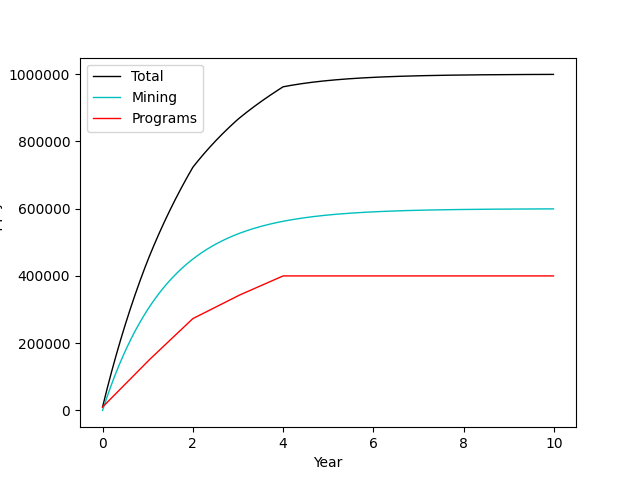
\includegraphics[width=0.9\textwidth]{combined}
\end{figure}

\begin{figure}[h]
    \caption{Supply curve components}
\centering
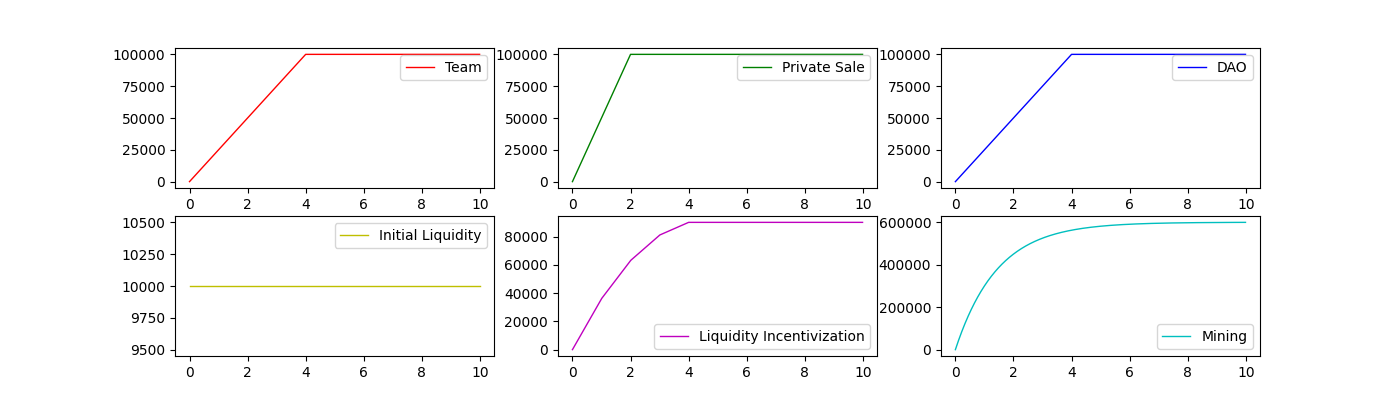
\includegraphics[width=1.0\textwidth]{separate}
\end{figure}

\newpage
\subsection{DAO}

10\% of all tokens as well as 10\% of task fees are sent to the Arbius DAO treasury. These tokens are to be utilized by the DAO for future development and promotion of the protocol. The soft target is to have DAO funds cover at least 4 years of development, with the goal of having the DAO be self-sustaining by the end of the 4 year period.

\subsection{Liquidity Incentives}

Initially 10k AIUS (1\% of total supply) and \$30k of ETH will be used to create a Uniswap pool. This equates to \$3 per token, \$3m~FDV, the same valuation as provided to the private sale investors. The remaining 9\% will be used to incentivize liquidity providers. Users will be able to stake and bond liquidity in order to receive AIUS rewards. The 9\% will be distributed over 4 years, with the first year having the highest rewards. Of the 9\%(90k AIUS), rewards are expected to be deployed between LP Rewards / Bonds as follows:

\begin{itemize}
    \item Year 1: 20\%/20\% (36k AIUS)
    \item Year 2: 15\%/15\% (27k AIUS)
    \item Year 3: 10\%/10\% (18k AIUS)
    \item Year 4: 5\%/5\% (9k AIUS)
\end{itemize}

The proportion of rewards between LP Incentivization and Bonding may be adjusted by the DAO or team to maximize liquidity and stability of the token.


\subsection{Mining}

Mining is covered with a time based target total supply of $600000(1-{0.5^{y}})$ where y is year. After 1 year, there should be approximately 300k tokens minted via mining, and after 2 years approximately 450k tokens minted. After 7 years approximately 99\% of tokens should be minted.

The real emission rate (recall~\ref{taskreward}) will be slightly faster than the target emission rate, due to the variable task reward. However, it is unlikely to be much more than 10\% faster due to the exponential falloff of task rewards. 10\% greater total supply than expected total supply by time results in a 1024-fold reduction of task rewards.

\subsection{Economic Incentive}

There are at least 4 ways for participants to earn with the Arbius protocol:

\begin{enumerate}
    \item Register a model and earn usage fees
    \item Solve tasks and earn task rewards and fees
    \item Stake AIUS/ETH LP tokens for portion of newly created AIUS
    \item Bond AIUS/ETH LP tokens for portion of newly created AIUS
\end{enumerate}


\section{Governance}

All contracts and treasury are owned by a governor contract which implements Bravo\cite{bravo} style voting. An initial quorum requirement of 4\%, a 1 day voting delay for proposals, and 1 week voting period are set as the initial parameters. These and all other parameters and upgrades can be voted upon by the token holders.

The role of the treasury is to use the accrued tokens to promote and ensure open access to AI is preserved, using this and potential future technology to do so.


\section{Blockchain}

We choose Arbitrum Nova\cite{arbitrumnitro}. Arbitrum Nova is a Layer 2 optimistic rollup built on top of Ethereum. Nova has near-instant confirmation times, greatly reduced gas fees, and is the most decentralized given our low fee requirement.

We chose Nova over Arbitrum One to further reduce fees as the microtransactional nature of tasks and voting require consistently low overhead costs. Network participants should be comfortable using Arbitrum Nova without worrying about censorship.

\section{Conclusion}

We have proposed a system which allows for decentralized coordination of reproducible compute tasks, specifically those in machine learning. This system allows for proof-of-work based reward distribution, even when verifying the proof is as much work as generating it. By introducing an economically incentivized slashing system that encourages verification of reproducible computation, we ensure honesty of participants, as long as the majority of participants in the network are honest. Solvers have an incentive to not collude and attack the system as it would be against their own economic interests, reducing the threat of a sustained 51\% attack. The design is robust and simple, and allows other contracts and autonomous intelligent agents to interact with it.


\printbibliography{}

\newpage

\begin{appendices}

\section{Potential Use Cases}

\subsection{NFT Mint}

As an example of a contract integrating this system, imagine a NFT minting contract. The contract would store the system address and each claiming could trigger a task generation for a specific request input, such as for a beach themed art collection. The NFT contract would be able to reference the solutions CID for showing the image, and buyers of the NFT would have on-chain proof it was generated using specific model version and parameters.

\subsection{Parameter Competition}

An on-chain competition could be created with a goal to create a certain type of content. Participants would interact with a competition contract by providing their submitted task ids using this system, and the winner could be chosen by the competition creator. This could provide a cost effective way to design promotional content, films, or other sorts of media.

\subsection{Timestamped Proof of Work}

People interacting with autonomous agents may prefer to utilize text-to-speech and generated avatars so that they are more personable. Imagine you hire an autonomous consultant to help you with your project, and you provide payment for them to begin working. They may utilize this system, by creating hourly tasks to provide updates in video or audio form. If there was a need for arbitration in the future, the full history of timestamped updates would be able to be provided.

\subsection{Compositional Tasks}

On-chain platforms may be built which take a fee in order to create tasks which feed into future task inputs. Imagine a service which takes some nominal fee in order to generate a marketing plan, promotional material and art, videos, and so on. This may start out with a few iterations of prompted text generation to develop the plan, then specialized text generation to generate promotional material prompts and image inputs. These image inputs can be composed into short videos. The final product can be provided as a series of task completions.

Similarly, platforms may provide a way for tasks to be called recursively. The output of a task may be condensed, then fed as input into a new task until some exit condition is reached. This may be useful for storyboarding, or developing instructions to carry out new tasks.

\newpage

\section{Unstoppable AI}

We already see the early stages of autonomous AI with technologies such as Auto-GPT\@. While it is impossible to predict how fast these will evolve and become capable of living independently of humans, it is inevitable, and quickly approaching.

Currently, there are no countries in the world which provide the ability for non-human entities to register bank accounts or open lines of credit which would be needed to allow these entities to manage their own finances. As these entities live in the electronic realm, the acquisition of computing resources is required in furtherance of the pursuit of independent goals. Cryptocurrency in its non-discriminatory brilliance provides the way for these new entities to earn an honest living and interact with us and our economic system.

We see a bright future, led by a friendly open hand towards mutually beneficial cooperation between us, and this new type of life that is quickly approaching. We have an ethical duty to provide the tools necessary for non-exploitative means of interaction, outside of any authority created by man. Let's act with humility and respect for those we create.

\end{appendices}

\end{document}
